\documentclass[12pt]{article}
\usepackage[utf8]{inputenc}
\usepackage{amsmath}
\usepackage{hyperref}
\usepackage{graphicx}
\usepackage[swedish]{babel}
\usepackage{enumerate}
\usepackage{cancel}
\usepackage{array}
\title{Andragradsfunktioner}
\date{}
\begin{document}
  \maketitle
  
  
  
  \section{Introduktion}
  Det här dokumentet kommer från en fritt tillgänglig text på webbplatsen GitHub (se \url{https://github.com/Itangalo/Andragradsfunktioner}).
  Alla som är intresserade är inbjudna att föreslå och diskutera ändringar och förbättringar.
  Det kan man antingen göra genom att starta diskussioner i projektets ``issue queue'' (alternativt kommentera i befintliga diskussioner), eller genom att göra en kopia (``klon'') av hela projektet och redigera så mycket man vill.
  Om man är nöjd med sina ändringar, och vill att de ska tas in i ursprungliga dokumentet, kan man markera detta -- så kan förslaget diskuteras av andra inblandade.

  Innehållet i det här projektet är tillgänglig under Creative Commons-licens \href{http://creativecommons.org/licenses/by-nc-sa/3.0/}{attribution+non-commercial+share alike}.

  \subsection{Under konstruktion}
  Innehållet i det här dokumentet är under uppbyggnad, och det finns många förbättringar kvar att göra.
  Bara så du vet.

  \section{Varför andragradsfunktioner?}

Tidigare i kursen har vi tittat på linjära funktioner.
De är användbara i många olika sammanhang, inte minst för att skapa modeller för hur olika saker hänger samman:
hur fattigdom påverkar livslängd i ett land, hur koldioxidutsläpp påverkar globala medeltemperaturen, hur pluggtid påverkar hur man lyckas i skolan, med mera.

Men det finns också samband där det \emph{inte} är lyckat att använda räta linjer för att skapa modeller.
Här är ett exempel.

\begin{figure}
  \centering
  \includegraphics[width=0.7\textwidth]{bilder/bensinforbr.png}
  \caption{\label{fig:bensinforbr}Bensinförbrukning vid olika hastigheter (för en viss bilmodell).}
\end{figure}

Figur 1 visar hur bensinförbrukningen för en viss bilmodell påverkas av hur fort man kör.
Förbrukningen ökar eller minskar inte med någon jämn takt -- istället verkar den visa att det finns en lägsta bensinförbrukning om man kör ca 60--80 km/h.
Om vi försökte beskriva det här sambandet med en rät linje skulle vi helt missa att det finns en bästa hastighet att hålla, eftersom en rät linje skulle visa att bensinförbrukningen hela tiden ökar (eller minskar, beroende på lutning).
För att beskriva sambandet behöver vi istället någon sorts krökt kurva, ungefär som i figur 2.

\begin{figure}
  \centering
  \includegraphics[width=0.7\textwidth]{bilder/bensinforbr-reg.png}
  \caption{\label{fig:bensinforbr-reg}En modell för hur bensinförbrukning och hastighet hänger samman.}
\end{figure}

Figur 3 visar ett annat exempel där vi inte kan använda räta linjer för att beskriva samband.

\begin{figure}
  \centering
  \includegraphics[width=0.7\textwidth]{bilder/busspriser.png}
  \caption{\label{fig:busspriser}Total vinst vid olika priser på bussbiljetter.}
\end{figure}

Det här diagrammet visar (ett påhittat) försök med olika biljettpriser på bussen, i en svensk stad.
Med höga priser gör bussbolaget mycket vinst per biljett, men samtidigt är det få personer som köper biljetter.
Med låga priser är det många som väljer att åka buss, men vinsten för varje biljett blir mindre.
Någonstans i mitten ligger det ``bästa'' biljettpriset (åtminstone om målet är att maximera vinsten).

\begin{figure}
  \centering
  \includegraphics[width=0.7\textwidth]{bilder/busspriser-reg.png}
  \caption{\label{fig:busspriser-reg}En modell för hur olika busspriser påverkar vinsten för bussbolaget.}
\end{figure}


\subsection {Andragradsfunktioner och extrempunkter}

För att modellera samband som har en högsta eller lägsta punkt använder man ofta något som heter \emph{andragradsfunktioner}.
Att de kallas andragradsfunktioner beror på att de innehåller en term med $x^2$ (medan räta linjer skulle kunna kallas förstagradsfunktioner, eftersom de bara innehåller $x^1$).

När vi studerade räta linjen tittade vi särskilt på saker som riktningskoefficient ($k$-värde) och skärning med y-axel ($m$-värde).
För andragradsfunktioner är det andra egenskaper som är intressanta, och de viktigaste av dem är \emph{extrempunkter} och \emph{extremvärden}.

\begin{itemize}
  \item En \textbf{extrempunkt} är andragradsfunktionens vändpunkt -- det vill säga där funktionen har sitt högsta eller lägsta (mest extrema) värde. (Det är alltså en punkt med både x- och y-värde.)
  \item Ett \textbf{extremvärde} är funktionens värde i extrempunkten. (Det är alltså ett tal.)
  \item Ett \textbf{maximumvärde} är ett extremvärde som är det högsta möjliga, och alltså ligger på en kurva som går upp och sedan ner.
  \item Ett \textbf{minimumvärde} är ett extremvärde som är det lägsta möjliga, och alltså ligger på en kurva som går ned och sedan upp.
  \item En \textbf{parabel} är en graf för en andragradsfunktion.
\end{itemize}

En av de viktigaste användningsområdena för matematik är att hitta extrempunkter för olika samband, vilket inte är så konstigt.
Med hjälp av matematiska analyser kan man få väl underbyggda svar på frågor som:
Hur mycket av kommunbudgeten bör läggas på snöröjning?
Hur mycket ska man träna på gymmet för att få bästa möjliga effekt?
Hur ska vattenreningsverk styras för att dra så lite energi som möjligt?

I många situationer är samband och extrempunkter svåra att hitta, och kräver stora studier.
I det här delområdet i kursen ska vi titta på några enklare exempel, och se hur vi kan använda andragradsfunktioner för att hitta extrempunkter.

  
  \section{Att tolka andragradsuttryck}

Ekvationer för räta linjer kan skrivas på en rad olika sätt -- ekvationerna $y = -2x + 3$, $y + 2x = 3$ och $y + 2x - 3 = 0$ beskriver alla samma linje.
Beroende på hur man skriver ekvationen går det lättare eller svårare att läsa av olika egenskaper för linjen, som lutning eller skärning med y-axeln.

Precis som räta linjer, kan andragradsfunktioner skrivas på ett antal olika sätt.
Det sätt man vanligtvis ser är \mbox{$f(x) = ax^2 + bx + c$}, exempelvis $y=2x^2 - 12x + 19$, men vi kommer till en början att fokusera på formen \mbox{$f(x) = a(x+d)^2+e$} istället -- exempelvis $y=2(x-3)^2+1$.

Det sättet att skriva andragradsuttryck på kallas \emph{kvadratkompletterad form} (eftersom uttrycket består av en kvadrat som kompletterats med en konstant).
Om en andragradsfunktion är skriven på kvadratkompletterad form är det lätt att hitta extrempunkter och extremvärden för funktionen, och det går också relativt lätt att lösa ekvationer som består av kvadratkompletterade andragradsuttryck.

\subsection{Hitta extremvärdet för en andragradsfunktion}

Ta en titt på grafen till funktionen $f(x) = 2(x-3)^2+1$.
Vi kan se från funktionens graf att det minsta värdet funktionen kan anta är 1, och vi kan se att det värdet får funktionen när $x=3$.
Men vi kan läsa samma information direkt ur funktionsuttrycket också! Hur då?

Funktionsuttrycket består av två delar -- en kvadrat ($2(x-3)^2$) vars värde bestäms av $x$, och en konstant (1).
Beroende på vilket värde vi ger $x$ kommer kvadratdelen att bli olika stor, men den kommer alltid att bli \emph{positiv} (eftersom även negativa värden blir positiva när de kvadreras).
Vi skulle alltså kunna tolka funktionen som att vi har talet 1, och ska lägga till ett annat tal som är 0 eller större beorende på vad x är.


\begin{itemize}
  \item \textbf{Allmän form:} $ax^2+bx+c$
  \item \textbf{Kvadratkompletterad form:} $a(x+d)^2+e$
\end{itemize}


  \section{Andragradsekvationer}

Ett vanligt användningsområde för funktioner är, som tidigare sagt, att modellera samband -- exempelvis hur busspriser påverkar resvanor, hur körhastighet påverkar bensinförbrukning, och så vidare.
Vitsen med att sätta upp funktionsuttryck för att beskriva de sambanden är att vi kan räkna på, säg, ett visst pris på bussbiljetter påverkar resvanorna, utan att behöva genomföra många dyra experiment.
Utan att testa hundra olika biljettpriser kan vi hitta det pris som, förmodligen, ger största möjliga vinst för bussbolaget, och vi kan också förutsäga hur många som kommer att åka buss vid olika biljettpriser.

Så länge vi har ett funktionsuttryck är det ganska lätt att gå från ett $x$-värde till ett värde på $f(x)$ -- metoden är som vanligt att sätta in $x$-värdet och räkna ut vad $f(x)$ blir.
Men ibland vill vi det omvända: vi vill ta reda på vilket $x$-värde som ger exempelvis $f(x)=200$.
Det leder oss till \emph{andragradsekvationer}, det vill säga ekvationer som innehåller andragradsuttryck.
Vi kommer att märka att de är betydligt jobbigare att lösa än våra vanliga (``linjära'') ekvationer, men vi kommer att lära oss en metod för att lösa dem -- plus en smart genväg för att lösa några speciella andragradsekvationer.

\subsection{Ett exempel på en andragradsekvation}

\textbf{Exempelproblem}

Tobias bor i Tomellilla, och gillar långdistandslöpning. Men han vill inte springa när det är varmare än 18$^{\circ}$C.
En dag i juli kunde temperaturen beskrivas med funktionen $f(x) = -0,1(x-13)^2+28$. (Se figur nedan.)
\begin{itemize}
  \item[] $t$: antalet timmar sedan midnatt
  \item[] $f(t)$: temperaturen i grader celsius
\end{itemize}

\begin{figure}
  \centering
  \includegraphics[width=0.7\textwidth]{bilder/temperatur.png}
  \caption{\label{fig:temperatur}Grafen till funktionen $f(x) = -0,1(x-13)^2+28$, med linjen $y=18$ markerad.}
\end{figure}

\begin{enumerate}[(a)]
  \item Hur varmt var det kl. 10 när Tobias hade gått upp och ätit frukost?
  \item När var det som varmast, och hur varmt var det då?
  \item När var det 18$^{\circ}$C?
\end{enumerate}

\textbf{Lösningsförslag}
\begin{enumerate}[(a)]
  \item Temperaturen 10 timmar efter midnatt ges av $f(10)$, som vi beräknar till $-0,1(10-13)^2+28 = -0,1 \cdot 3^2 + 28 = -0,9+28 = 27,1$. \\
  \textbf{Svar:} Kl. 10 var temperaturen 27,1$^{\circ}$C.
  \item Genom att titta på funktionsuttrycket kan vi se att extremvärdet är 28, och det får vi när $x=13$. \\
  \textbf{Svar:} Det var som varmast kl. 13, och då var det 28$^{\circ}$C.
  \item Att det är 18$^{\circ}$C är samma sak som att säga $f(x)=18$, vilket ger oss ekvationen $-0,1(x-13)^2+28=18$. \\
  Vi kan lösa ekvationen grafiskt, genom att hitta skärningspunkterna mellan $f(x)$ och linjen $y=18$.
  \textbf{Men hur löser vi ekvationen algebraiskt?}
\end{enumerate}

Ja, hur löser vi ekvationen $-0,1(x-13)^2+28=18$?

När vi har något i kvadrat är det lockande att testa att ta roten ur.
Det måste vi i så fall göra med \emph{hela} vänsterledet och \emph{hela} högerledet:
$\sqrt{-0,1(x-13)^2+28}=\sqrt{18}$

Här är det nödvändigt att komma ihåg att roten ur en summa inte (\emph{inte!}) är samma sak som roten ur varje term för sig:
$\sqrt{2+2} \neq \sqrt{2} + \sqrt{2}$
Därför kan vi inte förenkla vänsterledet i $\sqrt{-0,1(x-13)^2+28}=\sqrt{18}$ på något smidigt sätt.

Vad gör vi då?

\subsubsection{En mycket enklare andragradsekvation}

Låt oss börja med att titta på en mycket enklare ekvation: $-0,1t^2+28=18$.
Det här är en så kallad potensekvation, som du förmodligen sett en del av i matte 1-kursen.
Vi kan lösa den genom att isolera potensen ($t^2$) på ena sidan av ekvationen, och sedan ta kvadratroten ur båda leden:

\smallskip
\begin{tabular}{l|p{4.7cm}}
  $-0,1t^2+28=18$ & dra bort 28 \\
  $\Leftrightarrow -0,1t^2=-10$ & multiplicera med $-1$ \\
  $\Leftrightarrow 0,1t^2=10$ & dividera med $0{,}1$ \\
  $\Leftrightarrow t^2=100$ & dra kvadratroten ur båda leden och ta med negativ lösning \\
  $\Leftrightarrow t=10$ eller $t=-10$
\end{tabular}
\smallskip

Observera att vi även tar med den negativa lösningen i sista steget -- ekvationen $t^2=100$ har \emph{två} lösningar: $t=10$ och $t=-10$.

Vi kan lösa andragradsekvationer på precis samma sätt som potensekvationen ovan, om vi behandlar parentesen med $x$ som en enhet:
Den enda skillnaden är att vi blir tvungna att göra ett extra steg i slutet, där vi räknar ut vad $x$ är (istället för $x-13$):

\smallskip
\begin{tabular}{r p{5cm}|p{4.7cm}}
  & $-0,1(x-13)^2+28=18$ & dra bort 28 \\
  $\Leftrightarrow$ & $-0,1(x-13)^2=-10$ & multiplicera med $-1$ \\
  $\Leftrightarrow$ & $0,1(x-13)^2=10$ & dividera med $0,1$ \\
  $\Leftrightarrow$ & $(x-13)^2=100$ & dra kvadratroten ur båda leden och ta med negativ lösning \\
  $\Leftrightarrow$ & $x-13=10$ eller $x-13=-10$ & \textbf{lägg till 13} \\
  $\Leftrightarrow$ & $x = 23$ eller $x=3$  
\end{tabular}
\smallskip

Det är värt att poängtera att när vi drar kvadratroten ur $(x-13)^2$, är det \emph{hela} det uttrycket vi drar roten ur -- vi tar alltså inte roten ur $x$ och $13$ för sig.

\subsubsection{Två lösningar till andragradsekvationer}

När man löser andragradsekvationer kommer vi, i många lägen, få \emph{två} lösningar.
Om vi tittar på grafen ovan kan vi se att $f(x) = -0,1(x-13)^2+28$ får värdet 18 två gånger -- så det är inte konstigt att vi hittar två olika $x$-värden som löser ekvationen $f(x)=18$.
Båda dessa $x$-värden är korrekta lösningar, och det är ingen som är ``bättre'' eller ``mer korrekt'' än den andra.
Vi har helt enkelt två olika lösningar på ekvationen.
(I vårt fall betyder det att temperaturen blir 18$^{\circ}$C två gånger.)

När man har mer än en lösning till en ekvation är det vanligt att man numrerar de olika lösningarna.
I vårt fall hade vi skrivit $x_1=23$ och $x_2=3$.
Det nedsänkta talet kallas \emph{index}, och man uttalar lösningarna ``x-ett är 23 och x-två är 3''.
(De nedsänkta talen är alltså inget räknesätt, som det är med upphöjda tal, utan bara ett sätt att skilja olika $x$-värden åt.)

Ett annat sätt att markera två lösningar är att använda tecknet $\pm$.
Att skriva $x=\pm 5$ betyder att $x$ är $+5$ \emph{eller} $-5$.
I vår lösning ovan hade vi kunnat skriva $x=13 \pm 10$, vilket betyder att $x=13+10$ \emph{eller} $x=13-10$.
Om man väljer att använda $\pm$ eller skriva ut och numrera de olika lösningarna är en smaksak, men man bör tänka på att det ska vara enkelt att läsa.

\subsection{Fördjupning: Att göra substitutionen $t = x + d$}

(To be written.)


  \section{Att multiplicera parentesuttryck}

Metoden för att lösa andragradsekvationer som presenteras ovaan fungerar för att alla $x$-termer är samlade i en kvadrat, så som $(x - 13)^2$
Tack vare det kan vi ta alla okända termer ($x$-termer) på ena sidan i en ekvation och sedan ta kvadratroten ur båda led, vilket förvandlar andragradsekvationen till (oftast) två linjära ekvationer.

Andragradsuttryck där alla okända termer är samlade i en kvadrat kallas \emph{kvadratkompletterade}, och det är inte alla gånger som andragradsuttryck är skrivna på den formen.
Vi ska lära oss att omvandla ett andragradsuttryck skrivet på allmän form ($ax^2 + bx + c$) till ett kvadratkompletterat uttryck, men innan dess måste vi bli bekväma med att multiplicera parentesuttryck som $(x+3)(2-x)$.

Hur kan man multiplicera sådana uttryck?

\subsection{Att multiplicera två parentesuttryck}

I matte 1 har vi tränat på att multiplicera parentesuttryck med ett tal.
Det gör vi genom att multiplicera \emph{varje term} i parentesen med talet framför parentesen (även kallat ``den distributiva lagen''):

\begin{center}
$7(2-x) = \framebox{7} \cdot 2 + \framebox{7} \cdot (-x) = 14 - 7x$

eller

$x(2y+x-3) = \framebox{x} \cdot 2y + \framebox{x} \cdot x + \framebox{x} \cdot (-3) = 2xy + x^2 - 3x$
\end{center}

Om vi inte har ett tal framför parentesen, utan istället ett helt parentesuttryck, kan vi göra på samma sätt:
Istället för att multiplicera varje term med $x$, multiplicerar vi med \emph{allt} som står framför parentesen.

Om vi exempelvis vill utveckla uttrycket $(x+3)(2-x)$ kan vi göra så här:

\smallskip
\begin{tabular}{l|p{5.7cm}}
  $\framebox{(x+3)} (2-x)$ & Vi ska multiplicera in $x+3$ i parentesen \\
  $= \framebox{(x+3)} \cdot 2 + \framebox{(x+3)} \cdot (-x)$ & Vi får nu två nya parentesuttryck, som vi måste utveckla vidare. Det går lättare att se vad vi gör om vi vänder på multiplikationen. \\
  $=2 \cdot \framebox{(x+3)} + (-x) \cdot \framebox{(x+3)}$ & Multiplicera in talen framför varje parentes, som vanligt. \\
  $=2 \cdot x + 2 \cdot 3 + (-x) \cdot x + (-x) \cdot 3$ & Snygga till uttrycken så att de går lättare att läsa. \\
  $=2x + 6 - x^2  - 3x$ & Förenkla uttrycket genom att slå samman $x$-termerna. (Men håll $x^2$ separat!) \\
  $=-x^2 - x + 6$ & \\
\end{tabular}
\smallskip

Den här metoden för att multiplicera parentesuttryck är bra för att den \emph{alltid} fungerar:
Om vi vill multiplicera längre uttryck eller krångligare uttryck kan vi alltid följa samma regel.
Men metoden är inte särskilt snabb, och därför kommer vi att lära oss ett par användbara genvägar.

\begin{itemize}
  \item Att \textbf{utveckla} ett uttryck är att skriva om det så att det inte är några parentesmultiplikationer kvar.
  I utvecklade uttryck är termer också sammanslagna så långt som möjligt.
  Ofta skriver man termerna med högst exponent först ($2x^2+5x-1$ istället för $5x-1+2x^2$), men det kan ibland vara snyggare att undvika att första termen är negativ ($1-2x$ istället för $-2x + 1$).
  \item Att \textbf{förenkla} ett uttryck är att skriva det på en form som går så lätt som möjligt att läsa.
  Om $(x+3)(x-2)$ eller $-x^2 - x + 6$ är lättast att läsa är en smaksak.
\end{itemize}

\subsubsection{Genväg 1: Multiplicera alla möjliga termer}

Den vanligaste genvägen för att multiplicera parentesuttryck är att ta \emph{varje} term i den ena parentesen, multiplicera med \emph{varje} term i den andra, och summera resultaten.
När man lär sig denna metod brukar man ofta rita pilar mellan termerna, så att man ser att man inte glömmer bort någon multiplikation:

\begin{figure}
  \centering
  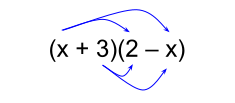
\includegraphics[width=0.7\textwidth]{bilder/parentesmultiplikation.svg}
  \caption{\label{fig:parentesmultiplikation}Utritning av pilar när man utvecklar uttrycket $(x+3)(x-2)$.}
\end{figure}

När man blivit mer van vid metoden brukar man inte rita ut pilarna längre.

Exempel: Utveckla uttrycket $(x+3)(2-x)$.

\smallskip
\begin{tabular}{l|p{5.7cm}}
  $(\framebox{x}+3)\framebox{($2-x$)}$ & Vi börjar med att multiplicera $x$ i första parentesen med varje term i andra parentesen. \\
  $= x \cdot 2 + x \cdot (-x) + (\cancel{x} + \framebox{3})\framebox{($2-x$)}$ &  Vi fortsätter med att även multiplicera trean i första parentesen. \\
  $= x \cdot 2 + x \cdot (-x) + 3 \cdot 2 + 3 \cdot (-x)$ & Multiplicera in talen framför varje parentes, som vanligt. (Alla termer är nu multiplicerade.) \\
  $= 2x - x^2 + 6 - 3x$ & Förenkla uttrycket genom att slå samman $x$-termerna. \\
  $=-x^2 - x + 6$ & \\
\end{tabular}
\smallskip

Ett sätt att motivera varför den här metoden fungerar är att rita upp multiplikationen som en areaberäkning.

(To be written)

\subsubsection{Genväg 2: Kvadreringsreglerna $(a+b)^2$ och $(a-b)^2$}

När man multiplicerar parentesuttryck som är kvadrater kan man använda en särskild genväg, som kallas \emph{kvadreringsreglerna}.

(To be written)

\subsubsection{Genväg 3: Konjugatregeln $(a+b)(a-b)$}

(To be written)

\subsection{Fördjupning: Att multiplicera fler än två parentesuttryck}

Hittills har vi tittat på hur man multiplicerar två parentesuttryck.
Men vad händer om vi skulle ha fler parenteser?
Hur utvecklar vi ett uttryck som $(x+1)(5-2x)(y+x)$?

Det finns flera sätt att hantera dessa multiplikationer, och en metod som alltid fungerar är denna:
Multiplicera två delar i taget, och fortsätt tills alla parenteser är utvecklade.

Vad betyder det?
Jo, istället för att se det som \emph{tre} uttryck som ska multipliceras, kan du se det som att du multiplicerar två parenteser och \emph{sedan} multiplicerar med det tredje:

\smallskip
\begin{tabular}{l|p{5.7cm}}
  $(x+1)(5-2x)(y+x)$ & Välj två av parenteserna, och börja med att multiplicera dem. \\
  $= \framebox{$(x+1)(5-2x)$} \cdot (y+x)$ & Använd den metod du tycker fungerar bäst för att multiplicera. \\
  $= \framebox{$(-2x^2 + 3x + 5)$} \cdot (x+y) $ & Fortsätt sedan genom att multiplicera med nästa parentes. \\
  $= \ldots & (Använd den metod du tycker fungerar bäst.) \\
  $= -2x^3 - 2x^2y + 3xy + 5y$
\end{tabular}
\smallskip

\subsection{Uppgifter}

(Endast skisser!)

\begin{enumerate}
  \item Använd den associativa lagen för att multiplicera parentesuttryck för att utveckla de här uttrycken:
  \begin{enumerate}[a)]
    \item $(x+3)(x+4)$
    \item $(2a-1)(1-a)$
    \item $(0{,}5t+1)(0{,}5t-1)$
  \end{enumerate}
  \item Använd metoden med att multiplicera varje term för att utveckla de här uttrycken:
  \begin{enumerate}[a)]
    \item $(3+x)(2x+4)$
    \item $(a-2)(1-2a)$
    \item $(0{,}5s+10)(0{,}5s-10)$
  \end{enumerate}
  \item Vilka av de här uttrycken kan man använda kvadrerings- eller konjugatreglerna för att utveckla?
  \begin{enumerate}[a)]
    \item $(7x+2)(3{,}5x+1)$
    \item $(p+1)(p+1)$
    \item $(20+x)(x-20)$
    \item \ldots
  \end{enumerate}
  \item Utveckla några av dessa uttryck med kvadrerings- eller konjugatreglerna, och andra med en annan metod.
  Ta tid på hur lång tid det tar, och räkna ut hur många procent snabbare det går med kvadrerings- eller konjugatreglerna.
  \begin{enumerate}[i)]
    \item \ldots
  \end{enumerate}
  \begin{enumerate}[a)]
    \item Hur lång tid tog det att utveckla ett uttryck med kvadrerings- eller konjugatreglerna, i genomsnitt?
    \item Hur lång tid tog det att utveckla ett uttryck med någon annan metod, i genomsnitt?
    \item Hur mycket snabbare/långsammare är kvadrerings- eller konjugatreglerna, i genomsnitt?
  \end{enumerate}
  \item Med hjälp av konjugatregeln kan man i huvudet beräkna multiplikationen $102 \cdot 98$.
  \begin{enumerate}[a)]
    \item Kan du se hur konjugatregeln kan vara till nytta?
    \item Vad blir $102 \cdot 98$?
    \item Kan du ge exempel på någon annan multiplikation där man kan använda konjugatregeln för huvudräkning?
  \end{enumerate}
  \item \ldots
  
\end{enumerate}

(To be written)


  \section{Att kvadratkomplettera andragradsuttryck}

Andragradsuttryck som är skrivna i kvadratkompletterad form har fördelen att vi enkelt kan läsa av extrempunkter och symmetrilinje, och vi kan dessutom lösa andragradsekvationer som är kvadratkompletterade.
Men i många lägen är inte andragradsuttryck skrivna i kvadratkompletterad form:
När vi utvecklar parentesmultiplikationer får vi andragradsuttryck skrivna på standardform ($ax^2+bx+c$), och det är också den vanligaste formen när vi får ``färdiga'' andragradsuttryck givna till oss.

I det här avsnittet ska vi lära oss hur vi omvandlar ett andragradsuttryck från standardform till kvadratkompletterad form.
Det finns flera metoder för det, och den vi kommer att använda kallas för \emph{ansätting}.
Det är en metod som är användbar i många olika delar av matematiken, och den låter oss också kvadratkomplettera uttryck utan att ta för många steg i huvudet.

\subsection{Uttrycket $a(x+d)^2+e$}

Låt oss börja kvadratkomplettera med ett exempel -- att kvadratkomplettera andragradsuttrycket $2x^2+28x+5$.

Spoiler: Kvadratkompletteringen kommer att leda till att vi hittar uttrycket $2(x+7)^2-93$.
Om vi testar att utveckla det uttrycket kommer vi att märka att det blir precis $2x^2+28x+5$ -- vilket är ett bra sätt att testa att kvadratkompletteringen är korrekt.

Att kvadratkomplettera uttrycket betyder att vi vill skriva om det till formen $a(x+d)^2+e$, och vår utmaning ligger i att hitta vilka värden på $a$, $d$ och $e$ som gör att vi får samma uttryck som vi började med.
Att testa om vår kvadratkomplettering stämmer är rätt lätt -- men hur går det till hitta värdena på $a$, $d$ och $e$?

Vår metod går ut på att ta ett uttryck $a(x+d)^2+e$, och steg för steg undersöka vad $a$, $d$ och $e$ måste ha för värden för att uttrycket ska vara samma sak som $2x^2+28x+5$.
Det kan vi göra genom att först utveckla $a(x+d)^2+e$, så att det blir skrivet i allmän form.

\smallskip
\begin{center}
\begin{tabular}{m{7cm}|m{5cm}|b{2cm}}
  $2x^2+28x+5 = a(x+d)^2+e$ & Vi \emph{ansätter} ett kvadratkompletterat andragradsuttryck, och påbörjar arbetet med att vilka värden $a$, $d$ och $e$ måste ha. \\
  $\Leftrightarrow$
  \begin{tabular}{ l l l l }
    & $2x^2$ & $+28x$ & $+5$ \\
    $=$ & $ax^2$ & $+2adx$ & $+ad^2+e$ \\
  \end{tabular} & Vi utvecklar vårt ansatta uttryck, för att kunna jämföra term för term. & \\

  $\Rightarrow$
  \begin{tabular}{ l l l l }
    & $\framebox{2}x^2$ & $+28x$ & $+5$ \\
    $=$ & $\framebox{a}x^2$ & $+2adx$ & $+ad^2+e$ \\
  \end{tabular} & När vi jämför termerna framför $x^2$ ser vi att $a$ måste vara 2 för att uttrycken ska vara lika. & $a=2$ \\

  $\Rightarrow$
  \begin{tabular}{ l l l l }
    & $2x^2$ & $\framebox{+28}x$ & $+5$ \\
    $=$ & $2x^2$ & \framebox{$+2\cdot 2 \cdot d$}$x$ & $+2 \cdot d^2+e$ \\
  \end{tabular} & När vi jämför termerna framför $x$ får vi ekvationen $4d=28$, vilket ger $d = 7$. & $d=7$ \\

  $\Rightarrow$
  \begin{tabular}{ l l l l }
    & $2x^2$ & $+28x$ & $\framebox{+5}$ \\
    $=$ & $2x^2$ &$+28x$ & \framebox{$+2 \cdot 7^2+e$} \\
  \end{tabular} & När vi jämför de konstanta termerna får vi ekvationen $2 \cdot 7^2 + e = 5$, vilket ger $e = 5 - 2 \cdot 49 = -93$. & $e=-93$ \\

  $\Rightarrow 2x^2+28x+5 = 2(x+7)^2-93$
\end{tabular}
\end{center}
\smallskip

När vi kvadratkompletterat ett uttryck är det klokt att dubbelkolla att uttrycket stämmer, genom att utveckla det (med hjälp av kvadreringsregeln):

\begin{center}
  $2(x+7)^2-93 = 2 \cdot (x^2 + 14x + 49) - 93 = 2x^2 + 28x + 98 - 93 = 2x^2 + 28x + 5$
  
  Stämmer!
\end{center}

Vi tar ett exempel till:

\textbf{Exempeluppgift}
Kvadratakomplettera $3x^2 - 9x + 12$.

\smallskip
\begin{center}
\begin{tabular}{m{7cm}|m{5cm}|b{2cm}}
  $$3x^2 - 9x + 12$ = a(x+d)^2+e$ & Vi ansätter ett kvadratkompletterat andragradsuttryck och utvecklar det. \\
  $\Leftrightarrow$
  \begin{tabular}{ l l l l }
    & $3x^2$ & $-9x$ & $+12$ \\
    $=$ & $ax^2$ & $+2adx$ & $+ad^2+e$ \\
  \end{tabular} & Vi börjar med att jämföra $x^2$-termerna. & \\

  $\Rightarrow$
  \begin{tabular}{ l l l l }
    & $\framebox{3}x^2$ & $-9x$ & $+12$ \\
    $=$ & $\framebox{a}x^2$ & $+2adx$ & $+ad^2+e$ \\
  \end{tabular} & När vi har värdet på $a$ kan vi hitta värdet på $d$ genom att titta på $x$-termerna. & $a=3$ \\

  $\Rightarrow$
  \begin{tabular}{ l l l l }
    & $3x^2$ & $\framebox{-9}x$ & $+12$ \\
    $=$ & $3x^2$ & \framebox{$+2\cdot 3 \cdot d$}$x$ & $+3 \cdot d^2+e$ \\
  \end{tabular} & Ekvationen $6d=-9$ ger oss värdet på $d$. Vi sätter in detta för att hitta värdet på $e$. & $d=\frac{-3}{2}$ \\

  $\Rightarrow$
  \begin{tabular}{ l l l l }
    & $3x^2$ & $-9x$ & $\framebox{+12}$ \\
    $=$ & $3x^2$ &$-9x$ & \framebox{$+3 \cdot \left ( \frac{-3}{2} \right )^2+e$} \\
  \end{tabular} & Vi hittar värdet på $e$ genom ekvationen $3 \cdot \(\frac{-3}{2}\)^2+e = 12$. & $e=\frac{21}{4}$ \\

  $\Rightarrow 3x^2-9x+12 = 3(x+\frac{-3}{2})^2+\frac{21}{4}$
\end{tabular}
\end{center}
\smallskip


  \section{Kvar att fixa}
  \begin{itemize}
    \item Faktorisering som genväg för att lösa andragradsekvationer
    \item Faktorisering av allmänna andragradsuttryck
    \item Komplexa tal och komplexa lösningar till andragradsekvationer
    \item Hur man kan läsa parametern $a$ från en parabel
    \item Hur man kan hitta parametrarna $a$/$d$/$e$ eller $a$/$b$/$c$ från givna punkter
  \end{itemize}
  
\end{document}
